\documentclass[11pt]{article}
\usepackage[margin=1in]{geometry}
\usepackage{graphicx}
\usepackage{amsmath}
\usepackage{amssymb}
\usepackage{float}
\usepackage{subcaption}
\usepackage{booktabs}

\title{Meeting Document}

\begin{document}
\maketitle

\section{$c_d$ Estimation}
  For the $c_d$ estimation, we first top code the sentences observed in the data to 720 months, following the convention of Hester 2017. This only affects $0.004$ of all cases (82/17,516). We then use this top coded sentence to compute each $\tau_i$. We also use our data to compute $\theta_i$ for each defendant. We use these two quantities, along with the top coded sentence variable, to create the convex hull for the judges. Once we have the convex hull for each judge, we use it to compute $l_j(\theta_i \tau_i)$ and $u_j(\theta_i \tau_i)$ for each defendant. We then use this information to split the defendants into three groups as specified by the write up. We calculate the overall negative log likelihood (i.e. we sum the negative log likelihood of each individual defendant) and then minimize this quantity (subject to the constraint that the expected number of trials matches the data) using a black box optimizer. We add $\epsilon=0.00001$ to each likelihood before taking the log to avoid taking the log of 0. The optimization algorithm is sensitive to the initialization and to the value of $\epsilon$. There are some initializations and values of $\epsilon$ for which the algorithm won't terminate successfully, and it will return the message "Desired error not necessarily achieved due to precision loss". We ran the optimization procedure with different values of $\epsilon$ and with different random initializations. For the random initializations, $\pi$ was initialized to a random number between 0 and 1, and $\mu_1, \sigma_1, \mu_2, \sigma_2$ were all initialized to different random numbers between 2 and 25. The results of the estimation can be found in the attached csv file. 

\section{$c_d$ Estimation Histograms}
  The figure below contains the following histograms: 
  \begin{itemize}
      \item Histogram of $c_d(i) = s_i - \hat{\theta_i}\hat{\tau_i}$ for $s\in \mathcal{I}_1$
      \item Histogram of $(u_i - \hat{\theta_i}\hat{\tau_i})$ for $s\in \mathcal{I}_2$
      \item Histogram of $(l_i - \hat{\theta_i}\hat{\tau_i})$ for $s\in \mathcal{K}$
      \item Histogram of all the above quantities combined. 
  \end{itemize}

  \begin{figure}[H]
      \centering
      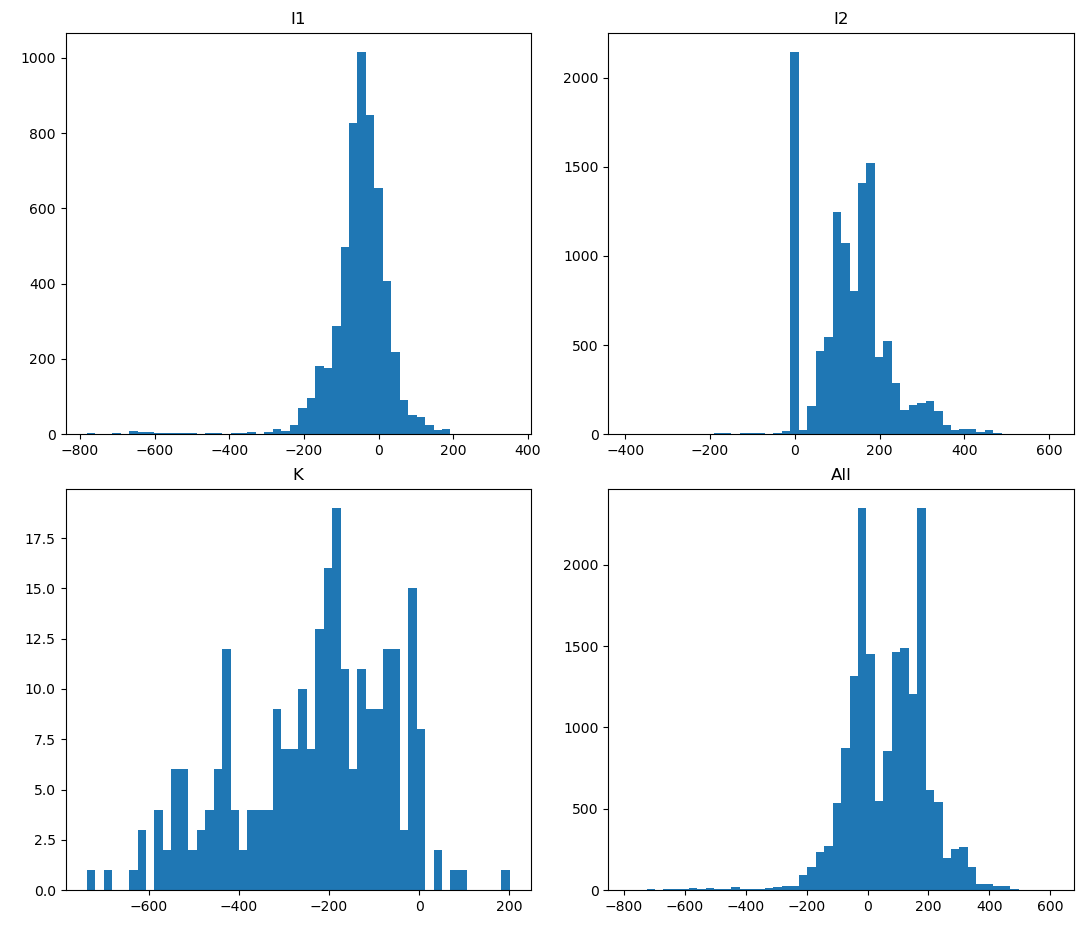
\includegraphics[width=0.75\textwidth]{../../../output/figures/Description/cd_histograms.png}
  \end{figure}

\end{document}